\documentclass[11pt,letterpaper]{article}

\newenvironment{proof}{\noindent{\bf Proof:}}{\qed\bigskip}

\newtheorem{theorem}{Theorem}
\newtheorem{corollary}{Corollary}
\newtheorem{lemma}{Lemma} 
\newtheorem{claim}{Claim}
\newtheorem{fact}{Fact}
\newtheorem{definition}{Definition}
\newtheorem{assumption}{Assumption}
\newtheorem{observation}{Observation}
\newtheorem{example}{Example}
\newcommand{\qed}{\rule{7pt}{7pt}}

\newcommand{\solution}[4]{
\thispagestyle{plain} 
\newpage
\setcounter{page}{1}
\noindent
\begin{center}
\framebox{ \vbox{
\vspace{4mm}
\vspace{0.2in} 
{\centering \large\mbox{#3}}\\
\vspace{0.1in}
{#1 \hfill {Date: #2}}
}}
\end{center}
\markright{#1}
}

\newenvironment{algorithm}
{\begin{center}
\begin{tabular}{|l|}
\hline
\begin{minipage}{1in}
\begin{tabbing}
\quad\=\qquad\=\qquad\=\qquad\=\qquad\=\qquad\=\qquad\=\kill}
{\end{tabbing}
\end{minipage} \\
\hline
\end{tabular}
\end{center}}

\def\Comment#1{\textsf{\textsl{$\langle\!\langle$#1\/$\rangle\!\rangle$}}}



\usepackage{graphicx, amssymb, amsmath, listings, float, mathtools}
\usepackage{color, url}
\lstset{language = Python}
\lstset{breaklines}
\lstset{extendedchars=false}

\oddsidemargin 0in
\evensidemargin 0in
\textwidth 6.5in
\topmargin -0.6in
\textheight 9.0in

\begin{document}

\solution{\large Jifu Zhao}{\large 11/18/2016}{\bf \Large ECE 544NA \hspace{0.5cm} 
		Fall 2016 \hspace{0.5cm} Assignment 5}

\section*{\Large TensorFlow}

\subsection*{\large 1. Methods}

\begin{description}

\item[(1) ] 
Note: In this section, we followed some online tutorials for the implemention problems, such as:
	\begin{description}
	\item[a.]$https://www.tensorflow.org/versions/r0.11/tutorials/recurrent/index.html$
	\item[b.]$https://tensorhub.com/aymericdamien/tensorflow-rnn$
	\item[c.]$https://github.com/tflearn/tflearn/blob/master/examples/images/rnn\_pixels.py$
	\item[d.]$https://github.com/tensorflow/tensorflow/blob/master/tensorflow/g3doc/api_docs/\\
				python/functions_and_classes/shard0/tf.nn.rnn.md$
	\end{description}
	
	
	


\item[(2) ] Limited by the computation resources, we didn't train too many iterations, especially for the model with $784$ steps. The detailed parameter settings are listed in Table \ref{table:parameter}.
\begin{table}[H]
	\centering
	\caption{Parameter settings}
	\label{table:parameter}	
	\begin{tabular}{c | c | c | c | c}
		\hline \hline
		Model 		  &	Basic RNN (t=784) & LSTM (t=784) &	Basic RNN (t=28) & LSTM (t=28) \\[0.1cm]
		\hline
		steps size	  &	784			  &	784			 	 &	28			 	 & 28 	 	   \\[0.1cm]
		input size	  &	1			  &	1			 	 &	28			     & 28		   \\[0.1cm]
		learning rate &	0.0005		  &	0.0001		 	 &	0.0001 		     & 0.0001	   \\[0.1cm]
		iterations	  &	2000		  &	1000		  	 &	5000 		     & 5000        \\[0.1cm]
		batch size	  &	100			  &	100			 	 &	100			     & 100		   \\[0.1cm]
		\hline	
	\end{tabular}
\end{table}


\end{description}


\subsection*{\large 2. Results}

\begin{description}

\item[(1) ] The convergence curves for mini-batch training-corpus accuracy of $4$ different models are shown in Figure \ref{fig:curve}.

\begin{figure}[H]
\centering
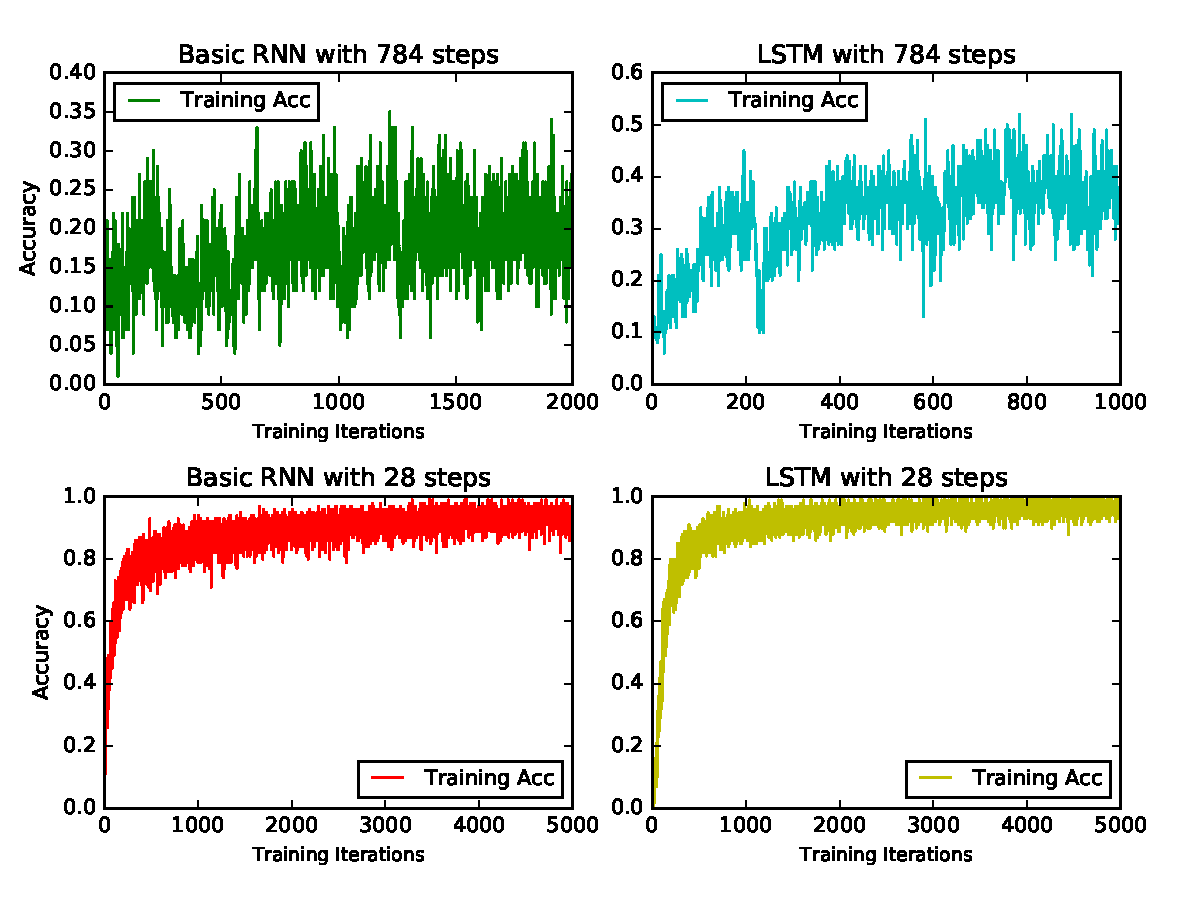
\includegraphics[width=1.0\textwidth]{./figures/convergence.pdf}
\caption{\label{fig:curve} Convergence Curve}
\end{figure}


\item[(2) ] The final training and testing accuracy are shown in Table \ref{table:accuracy}

\begin{table}[H]
	\centering
	\caption{Training and testing accuracies}
	\label{table:accuracy}	
	\begin{tabular}{c | c | c }
		\hline \hline
		Model 				&	Training Set	&  Testing Set \\[0.1cm]
		\hline
		Basic RNN (t=784) 	&	20.40\%			&  20.95\%     \\[0.1cm]
		LSTM (t=784)		&	40.82\%			&  40.76\%     \\[0.1cm]   
		Basic RNN (t=28)	&	93.61\%			&  94.20\%     \\[0.1cm]
		LSTM (t=28)			&	96.68\%			&  96.51\%     \\[0.1cm]
		\hline	
	\end{tabular}
\end{table}

\end{description}


\clearpage

%\bibliographystyle{plain}
%\bibliographystyle{unsrt}
%\bibliography{reference.bib}

\end{document}

